\documentclass[11pt, a4paper]{article}

\setlength\textwidth{145mm}
\setlength\textheight{247mm}
\setlength\oddsidemargin{15mm}
\setlength\evensidemargin{15mm}
\setlength\topmargin{0mm}
\setlength\headsep{0mm}
\setlength\headheight{0mm}
\let\openright=\clearpage

\usepackage[british]{babel}
\usepackage{lmodern}
\usepackage[T1]{fontenc}
\usepackage{textcomp}

\usepackage[utf8]{inputenc}

\usepackage{stddoc}
\usepackage{mathtools}
\usetikzlibrary{positioning}


\usepackage{titling}
\pretitle{\begin{center}\Huge\bfseries}
	\posttitle{\par\end{center}\vskip 0.5em}
\preauthor{\begin{center}\Large\ttfamily}
	\postauthor{\end{center}}
\predate{\par\large\centering}
\postdate{\par\vskip 5em}

\title{Tikz}
\author{Template document for learning purposes}
\date{}


\begin{document}
	
	\pagenumbering{arabic}
	
	\maketitle
	\thispagestyle{empty}
	
	\paragraph{Tikz package} is a powerful package allowing to draw pictures to visualise author's ideas.\\
	\textit{Note:} The tikzfigure environment can be enclosed inside a figure or similar environment.
	
	\subsection*{Geometric shapes}
		\begin{minipage}{0.4\textwidth}
			\begin{tikzpicture}
				\draw[gray, thick] (-1,2) -- (2,-4);
				\draw[gray, thick] (-1,-1) -- (2,2);
				\filldraw[black] (0,0) circle (2pt) node[anchor=west] {Intersection point};
			\end{tikzpicture}
		\end{minipage}
		\begin{minipage}{0.4\textwidth}
			\begin{tikzpicture}
				\draw (-2,0) -- (2,0);
				\filldraw [gray] (0,0) circle (2pt);
				\draw (-2,-2) .. controls (0,0) .. (2,-2);
				\draw (-2,2) .. controls (-1,0) and (1,0) .. (2,2);
			\end{tikzpicture}
		\end{minipage}
	
		\begin{tikzpicture}
			\filldraw[color=red!60, fill=red!5, very thick](-1,0) circle (1.5);
			\fill[blue!50] (2.5,0) ellipse (1.5 and 0.5);
			\draw[ultra thick, ->] (6.5,0) arc (0:220:1);
		\end{tikzpicture}
		
		\begin{tikzpicture}
			\draw[blue, very thick] (0,0) rectangle (3,2);
			\draw[orange, ultra thick] (4,0) -- (6,0) -- (5.7,2) -- cycle;
		\end{tikzpicture}
		
	
	\subsection*{Legend}
		
		\noindent
		We use \textbf{\textbackslash filldraw} for specifying outer and inner styles, \textbf{\textbackslash draw} when it's not needed.\\[3mm]
		\textbf{\textbackslash draw (-2,0) -- (2,0);} \dots defines a line with endpoints,\\
		\textbf{\textbackslash filldraw [gray] (0,0) circle (2pt);} \dots creates a gray point at a given location with given radius,\\
		\textbf{\textbackslash draw (-2,2) .. controls (-1,0) and (1,0) .. (2,2);} \dots draws a Beyiér curve with control points in the middle of the command (can be only one),\\
		\textbf{\textbackslash filldraw[color=red!60, fill=red!5, very thick](-1,0) circle (1.5);} \dots
		\begin{itemize}
			\item \textbf{color=red!60} \dots stets 60\% red for the outer ting,
			\item \textbf{fill=red!5} \dots fills the ring with 5\% red,
			\item \textbf{very thick} \dots thickness of the stroke (can be also used for the fill),
		\end{itemize}
		\textbf{\textbackslash fill[blue!50] (2.5,0) ellipse (1.5 and 0.5);} \dots defines an elipse with provided centre point and two radii,\\
		\textbf{\textbackslash draw[ultra thick, ->] (6.5,0) arc (0:220:1);} \dots draws an arc, where the last extra parameter \textbf{->} indicates an arrow at the end; provided are: centre point, starting angle, ending angle, radius \dots in format (x,y) arc (start angle, end angle, radius),\\
		\textbf{\textbackslash draw[blue, very thick] (0,0) rectangle (3,2);} \dots draws a rectangle, provided a starting point and a diagonal one,\\
		\textbf{\textbackslash draw[orange, ultra thick] (4,0) -- (6,0) -- (5.7,2) -- cycle;} \dots is a way of drawing a polygon (triangle here) while provided with individual points of the drawing path and the the \textbf{cycle} connects the last and the first point.
		
	\subsection*{Diagrams}
		
		\begin{tikzpicture} [
			roundnode/.style={circle, draw=green!60, fill=green!5, very thick, minimum size=7mm},
			squarednode/.style={rectangle, draw=red!60, fill=red!5, very thick, minimum size=5mm},
			]
			%Nodes
			\node[squarednode]      (maintopic)                              {2};
			\node[roundnode]        (uppercircle)       [above=of maintopic] {1};
			\node[squarednode]      (rightsquare)       [right=of maintopic] {3};
			\node[roundnode]        (lowercircle)       [below=of maintopic] {4};
		
			%Lines
			\draw[->] (uppercircle.south) -- (maintopic.north);
			\draw[->] (maintopic.east) -- (rightsquare.west);
			\draw[->] (rightsquare.south) .. controls +(down:7mm) and +(right:7mm) .. (lowercircle.east);
		\end{tikzpicture}
		
		\noindent
		Here, we essentially do main three processes: node declaration, node definition, drawing lines to connect the nodes:\\
		\textbf{roundnode/.style=\{circle, draw=green!60, fill=green!5, very thick, minimum size=7mm\}} \dots passes a circuitkz, which we're already familiar with, as a parameter to the declaration of a node later referred to as a \textit{roundnode}; \textit{squarenode} is created similarly,\\
		\textbf{\textbackslash node[squarednode] (maintopic) \{2\};} \dots creates a \textit{squarenode} as defined earlier with id \textit{maintopic} and will contain number 2 (no text if the parameter is left out),\\
		\textbf{[above=of maintopic]} \dots requires the \textbf{\textbackslash usepackage\{positioning\}} and sets the relative position of a node to a node specified by its id; it is possible to do without \textit{positioning} package by doing e.g. \textbf{of=maintopic} instead, but it is more flexible to do with it (e.g. allows to extend to \textbf{above=3cm of maintopic} to control the actual position from \textit{maintopic}),\\
		\textbf{\textbackslash draw[->] (uppercircle.south) -- (maintopic.north);} \dots draws an arrow-like (thanks to the addition \textbf{->} parameter) line as was explained before.
		
		\subsection*{Additional information}
			
			\noindent
			List of possibile values of the parameter \textbf{color}: white, black, red, green, blue, cyan, magenta, yellow;\\[2mm]
			List of possible values of the parameter \textbf{thickness}: ultra thin, very thin, thin, thick, very thick, ultra thick.
	
	
	
	
	
\end{document}